\begin{flushright} {\tiny {\color{gray} \tt pair\_crouzeixraviart1.tex}} \end{flushright}
%~~~~~~~~~~~~~~~~~~~~~~~~~~~~~~~~~~~~~~~~~~~~~~~~~~~~~~~~~~~~~~~~~~~~~~~~~~~~~~~~~~~~~~~~~~~~~~~~~~

This is the degree-1 Crouzeix–Raviart on a triangle. See \textcite{crra73} (1973). 

\begin{center}
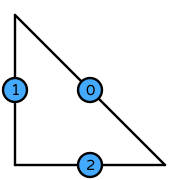
\includegraphics[width=3cm]{images/pair_crouzeix-raviart1/element-Crouzeix-Raviart-variant-equispaced-triangle-1-dofs}
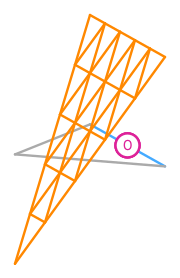
\includegraphics[width=2.5cm]{images/pair_crouzeix-raviart1/element-Crouzeix-Raviart-variant-equispaced-triangle-1-0}
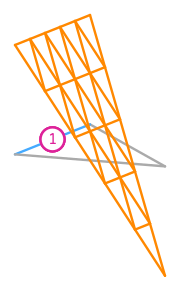
\includegraphics[width=2.5cm]{images/pair_crouzeix-raviart1/element-Crouzeix-Raviart-variant-equispaced-triangle-1-1}
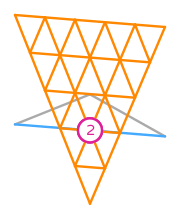
\includegraphics[width=3cm]{images/pair_crouzeix-raviart1/element-Crouzeix-Raviart-variant-equispaced-triangle-1-2}\\
{\captionfont Taken from https://defelement.com}
\end{center}

We find on the defelement page\footnote{\url{https://defelement.com/elements/examples/triangle-crouzeix-raviart-1.html}}
that the basis functions are given by:
\begin{eqnarray}
\bN_0(r,s)&=&2r+2s-1 \nn\\
\bN_1(r,s)&=&1-2r \nn\\
\bN_2(r,s)&=&1-2s \nn
\end{eqnarray}
We find $\bN_i(r_j,s_j)=\delta_{ij}$.

